\documentclass{article}

  \usepackage[letterpaper, top=1in, bottom=1in, left=1in, right=1in]{geometry}
  \usepackage[utf8]{inputenc}
  \usepackage[english]{babel}
  \usepackage{amsmath, amssymb, amsthm, mathrsfs, mathtools, centernot, hyperref, fancyhdr, lastpage}
  \usepackage{graphicx} 
  \usepackage{import}
  \usepackage{caption, subcaption}
  \usepackage{enumitem}
  \usepackage{fancyvrb,newverbs,xcolor}
  \definecolor{cverbbg}{gray}{0.93}

  \renewcommand{\thispagestyle}[1]{}

  \theoremstyle{definition}
  \newtheorem{theorem}{Theorem}[section]
  \newtheorem{proposition}[theorem]{Proposition}
  \newtheorem{lemma}[theorem]{Lemma}
  \newtheorem{example}{Example}[section]
  \newtheorem{exercise}{Exercise}[section]
  \newtheorem{corollary}{Corollary}[theorem]
  \newtheorem{definition}{Definition}[section]
  \renewcommand{\qed}{\hfill$\blacksquare$}
  \renewcommand{\footrulewidth}{0.4pt}% default is 0pt

  \newenvironment{solution}{\noindent \textit{Solution.}}{}

  \newenvironment{cverbatim}
   {\SaveVerbatim{cverb}}
   {\endSaveVerbatim
    \flushleft\fboxrule=0pt\fboxsep=.5em
    \colorbox{cverbbg}{%
      \makebox[\dimexpr\linewidth-2\fboxsep][l]{\BUseVerbatim{cverb}}%
    }
    \endflushleft
  }

  \newcommand{\incfig}[2][1]{%
    \def\svgwidth{#1\columnwidth}
    \import{./fig/}{#2.pdf\_tex}
  }

\begin{document}
\pagestyle{fancy}

\lhead{Computer Systems}
\chead{Muchang Bahng}
\rhead{\date{Spring 2024}}
\cfoot{\thepage / \pageref{LastPage}}


\title{Linux}
\author{Muchang Bahng}
\date{Spring 2024}

\maketitle

\tableofcontents

\pagebreak

The global variables are stored in the data. In the first slide, $i$ is a global variable and it gets copied onto the stack for the function call. 
Strings, which are arrays of chars, can be initialized by arrays or string literals. 

\section{Memory Management} 

  Let's talk about memory, which can be visualized as a long array of ``boxes'' that each contain a byte. Now each box contains an address, which is usually represented as a hexadecimal, but ultimately it is encoded as sequence of bits. 

  A good thing to keep in mind is that: 
  \begin{enumerate} 
    \item A bit is a bit. 
    \item A hex is 4 bits. 
    \item A byte is 2 hex, or 8 bits. 
  \end{enumerate}

  There are usually two types of machines that tend to format these boxes very differently: 32-bit and 64-bit machines. The numbers typically mean the size of the type that the machine works best with, so all memory addresses will be 32 or 64 bits wide. Most machines are 64-bits, so let's work with them (means 16 digit hexadecimal addresses). 

  \begin{cverbatim} 
    ...
    0x00007FFF7FBFF860 --> 0b000000000000000000000000011111111111
                           111101111111101111111111100001100000
    0x00007FFF7FBFF861 --> 0b000000000000000000000000011111111111
                           111101111111101111111111100001100001
    0x00007FFF7FBFF862 --> 0b000000000000000000000000011111111111
                           111101111111101111111111100001100010
    0x00007FFF7FBFF863 --> 0b000000000000000000000000011111111111
                           111101111111101111111111100001100011
    0x00007FFF7FBFF864 --> 0b000000000000000000000000011111111111
                           111101111111101111111111100001100100
    ...
  \end{cverbatim}

  Therefore, everything is stored in these memory addresses, and we can verify it for ourselves. In here, these memory addresses are presented in 12 digit hexadecimals, but that is because it doesn't print the leading 0s. 

  \begin{cverbatim} 
    int dummy_function(int input) {
      return input; 
    }

    int main(void) {
      int x = 4; 
      printf("%p", &x);               // 0x7ffdd4539c54 
      printf("%p", &dummy_function);  // 0x5c4d6c8ff16c
    }
  \end{cverbatim}

  CPUs also use these names. 32-bit processors have $2^{32}$ possible addresses in their cache, but 64-bit processors have a 48-address space. This is because CPU manufacturers took a shortcut. They use an instruction set which allows a full 64-bit address space, but current CPUs just only use the last 48-bits. The alternative was wasting transistors on handling a bigger address space which wasn't going to be needed for many years (since 48-bits is about 256TB).   

  \subsection{Bit Representation of Primitive Types}

    Let us talk about how we represent some of the simplest primitive types: unsigned short, unsigned int, unsigned long, unsigned long long.
    \begin{enumerate} 
      \item A short is 2 bytes long and can be represented as a 4-digit hex or 16 bits, with values in $[65,535]$. Therefore, say that we have 
        \begin{cverbatim} 
          0d15 = 0b1111 = 0x000F
        \end{cverbatim}

      \item An unsigned int is 4 bytes long and can be represented as an 8-digit hex or 32 bits, with values in $[4,294,967,295]$. 
      \item An unsigned long is 8 bytes and can be represented as an 16-digit hex or 64 bits, but they are only guaranteed to be stored in 32 bits in other systems. 
      \item An unsigned long long is 8 bytes and can be represented as an 16-digit hex or 64 bits, and they are guaranteed to be stored in 64 bits in other systems. 
    \end{enumerate} 

    So far, the process of converting unsigned numbers to bits seemed simple. However, when storing signed data types things become quite tricky. It is intuitive to simply take the first (left-most) bit and have that be the sign. Therefore, we lose one significant figure but gain information about the sign. However, this has some problems: first, there are two representations of zeros: $-0$ and $+0$. Second, the continuity from $-1$ to $0$ is not natural, since we represent $-1$ (say as a short) as 
    \begin{cverbatim} 
      0b1000000000000001
    \end{cverbatim}
    meaning that if we simply do binary operations on this, adding \texttt{0b1} to this will result in getting $-2$. Therefore, what we do is not have the first bit determine the sign of the rest of the bits (i.e. the entire number itself), but rather determine the sign of the most significant bit. Therefore, 
    \begin{cverbatim} 
      -1 = 0b1111111111111111 = 0xFFFF
    \end{cverbatim}

    This solves both problems and makes it more natural. 


    \begin{definition}[Endian Architecture]
      Depending on the machine architecture, computers may store these types slightly differently in their \textit{byte} order. Say that we have an integer of value \texttt{0xA1B2C3D4} (4 bytes). Then, 
      \begin{enumerate} 
        \item A \textbf{big-endian architecture} (e.g. SPARC, z/Architecture) will store it so that the least significant byte has the highest address.
        \item A \textbf{little-endian architecture} (e.g. x86, x86-64, RISC-V) will store it so that the least significant byte has the lowest address. 
        \item A \textbf{bi-endian architecture} (e.g. ARM, PowerPC) can specify the endianness as big or little. 
      \end{enumerate}

      \begin{figure}[hbt!]
        \centering 
        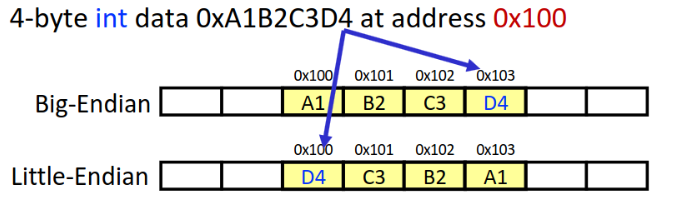
\includegraphics[scale=0.4]{img/endianness.png}
        \caption{The big vs little endian architectures. } 
        \label{fig:endianness}
      \end{figure}
    \end{definition}

    Now we can talk about the 

  \subsection{Pointers}

    Now when we define any variable, it must be stored in some memory address. This address is located somewhere in memory, and we can just add a asterisk sign before the variable name to determine where it is. It is of \textit{pointer} type, so we must print it with \texttt{\%p}. 

    \begin{cverbatim} 
      int main(void) {
        int x = 4; 
        printf("%p\n", &x); 
        return 0; 
      }
    \end{cverbatim}

    Since a pointer really stores a memory address, in a 64-bit architecture, the size of it should really be 8 bytes. Indeed this is the case. 

    \begin{cverbatim} 
      printf("%lu", sizeof(int*))   // 8
    \end{cverbatim}

    If we wanted to store this address in a variable, C provides \textit{pointer variables} which stores addresses to a specific type. Once a pointer is initialized, we can put a asterisk in front of it to get the value of what the pointer points to. We can initialize a pointer in multiple ways: 
    \begin{enumerate} 
      \item First define a variable of a certain type and initialize a pointer to point to that variable. The type that the pointer refers to should be what you initialize the pointer as. 
        \begin{cverbatim} 
          int x = 4; 
          int *p = &x; 

          // or 
           
          int x; 
          int *p = &x; 
          *p = 4; 
        \end{cverbatim}

      \item You can define a \textit{null pointer} which is simply an initialized pointer but it doesn't know the type that it will point to. You then have it point to the memory address of the integer variable, and then you can print out its contents by typecasting the void pointer to an int pointer, and then asterisking again to get its value as an int. 

      \begin{cverbatim} 
        void *p; 
        int x = 4; 
        p = &x; 
        printf("%d", *((int*)p)); 
      \end{cverbatim}
    \end{enumerate}


    \subsubsection{Pointer Arithmetic} 

      The great thing about pointers is that when you are allocating memory in the heap, you can access each array element easily. For example, 

      \begin{cverbatim} 
int main(void) {

  // initialize array 
  int arr[5]; 
  for (int val = 1; val < 6; val++) {
    arr[val-1] = val * val;
  }

  int* p = &arr[0]; 
  for (int i = 0; i < 5; i++) {
    printf("Value at position %d : %d\n", i, arr[i]); 
    printf("Address at position %d : %p\n", i, p + i); 
  }

  return 0; 
}        

Value at position 0 : 1
Address at position 0 : 0x7ffd8636b0d0
Value at position 1 : 4
Address at position 1 : 0x7ffd8636b0d4
Value at position 2 : 9
Address at position 2 : 0x7ffd8636b0d8
Value at position 3 : 16
Address at position 3 : 0x7ffd8636b0dc
Value at position 4 : 25
Address at position 4 : 0x7ffd8636b0e0

      \end{cverbatim}

  \subsection{Type Casting}



  \subsection{Global, Stack, and Heap Memory}

    When a program runs, its application memory consists of four parts: 

    \begin{enumerate} 
      \item The \textbf{code} is where the code text is stored. 
      \item The \textbf{global memory} is where all the global variables are stored. 
      \item The \textbf{stack} is where all of the functions and local variables are stored. 
      \item The \textbf{heap} is variable and can expand to as much as the RAM on the current system. We can specifically store whatever variables we want in the heap.
    \end{enumerate}

    Let's elaborate more on these four parts, and as a visual we will extend on the previous image of our memory, by dividing it into chunks. 

    \begin{figure}[ht]
      \centering
      \incfig{stack_heap_1}
      \caption{The application memory, can be thought of as the original memory as a long table of memory addresses. }
      \label{fig:stack_heap_1}
    \end{figure}

    The text is self explanatory, so let's focus on the stack and the global memory sections first. First, all global variables defined in your file will be put into the global memory. Simple enough. 

    Then, when you initialize any functions or local variables within those functions (which will be the majority of your code), all these will be stored in the stack, which is an literally an implementation of the stack data structure. It is LIFO, and the first thing that goes in is the \texttt{main} function and its local variables, which is referred to as the \textbf{stack frame}. You can't free memory in the stack unless its in the top of the stack. 

    Say that you have the following code: 

    \begin{cverbatim} 
      int total; 
      int Square(int x) {
        return x*x; 
      }
      int SquareOfSum(int x, int y) {
        int z = Square(x + y); 
        return z; 
      }
      int main() { 
        int a = 4, b = 8;              
        total = SquareOfSum(a, b); 
        printf("output = %d", total); 
        return 0; 
      }
    \end{cverbatim}
    
    The memory allocation of this program will run as such: 
    \begin{enumerate} 
      \item The \texttt{total} variable is initialized and is put into global memory. 
      \item \texttt{main} is called. It is put into the stack. 
      \item The local variables \texttt{a=4} and \texttt{b=8} are initialized and are put into the stack. 
      \item The \texttt{SquareOfSum} function is called and put into the stack. 
      \item The input local variables \texttt{x=4}, \texttt{y=8}, \texttt{z} are initialized and put into the stack. 
      \item \texttt{x + y=12} is computed and put into the stack. 
      \item The \texttt{Square} function is called and put into the stack. 
      \item The \texttt{x=12} local variable of \texttt{Square} is initialized and put into the stack. 
      \item The CPU computes \texttt{x*x=144} and returns the output. The \texttt{Square} function is removed from the stack. 
      \item We assign \texttt{z=144} and \texttt{SquareOfSum} returns it. Now \texttt{SquareOfSum} is removed from the stack. 
      \item \texttt{total=144} is assigned in the global memory still. 
      \item The \texttt{printf} function is called and put into the stack. 
      \item The \texttt{printf} function prints the output and is removed from the stack. 
      \item The \texttt{main} function returns \texttt{0} and is removed from the stack, ending our application. 
    \end{enumerate}

    One limitation of the stack is that its total available memory is fixed from the start, ranging from 1MB to 8MB, and so you can't initialize arrays of billions of integers in the stack. It will cause a memory overflow. In fact, the memory of the stack, along with the global and text memory, are assigned at compile time, making it a \textbf{static memory}. 

    Since the stack is really just a very small portion of available memory, the heap comes into rescue. The \textbf{heap memory} (nothing to do with the heap data structure) is a variable length (meaning it can grow at runtime) and \textbf{dynamically allocated} (meaning that we can assign memory addresses during runtime) memory that is limited to your computer's hardware. Unlike simply initializing variables to allocate memory as in the stack, we must use the \textbf{malloc} and \textbf{free} functions in C, and \textbf{new} and \textbf{delete} operations in C++. 

    Let's talk about how \texttt{malloc} and \texttt{free} are implemented in C. If you make a for loop and simply print all the addresses that you allocate to. You will find that they can be quite random. After a program makes some calls to malloc and free, the heap memory can becomes fragmented, meaning that there are chunks of free heap space interspersed with chunks of allocated heap space. The heap memory manager typically keeps lists of different ranges of sizes of heap space to enable fast searching for a free extent of a particular size. In addition, it implements one or more policies for choosing among multiple free extents that could be used to satisfy a request.

    The free function may seem odd in that it only expects to receive the address of the heap space to free without needing the size of the heap space to free at that address. That’s because malloc not only allocates the requested memory bytes, but it also allocates a few additional bytes right before the allocated chunk to store a header structure. The header stores metadata about the allocated chunk of heap space, such as the size. As a result, a call to free only needs to pass the address of heap memory to free. The implementation of free can get the size of the memory to free from the header information that is in memory right before the address passed to free.



    The stack can store pointer variables that point to the memory address in the heap. So the only way to access variables in the heap is through pointer reference, and the stack provides you that window to access that big pool of heap memory. 

    One warning: if you allocate another address, the previous address does not get deallocated off the memory. 



    At this point, we might be wondering why we need both a stack and a heap. Well the benefits of heaps are clearer since you can dynamically allocate memory, and you don't have the LIFO paradigm that is blocking you from deallocating memory that has been allocated in the beginning of your program. A problem with just having heap is that stacks can be orders of magnitude times faster when allocating/deallocating from it than the heap, and the sequence of function calls is naturally represented as a stack. 


\end{document}
